% Cardinality-repair follow-up (repo: Phase Y; replaces phase_y_cardinality_control.png).
%
% Usage: see externalization_protocol.tex for the required preamble.
% Replace the existing 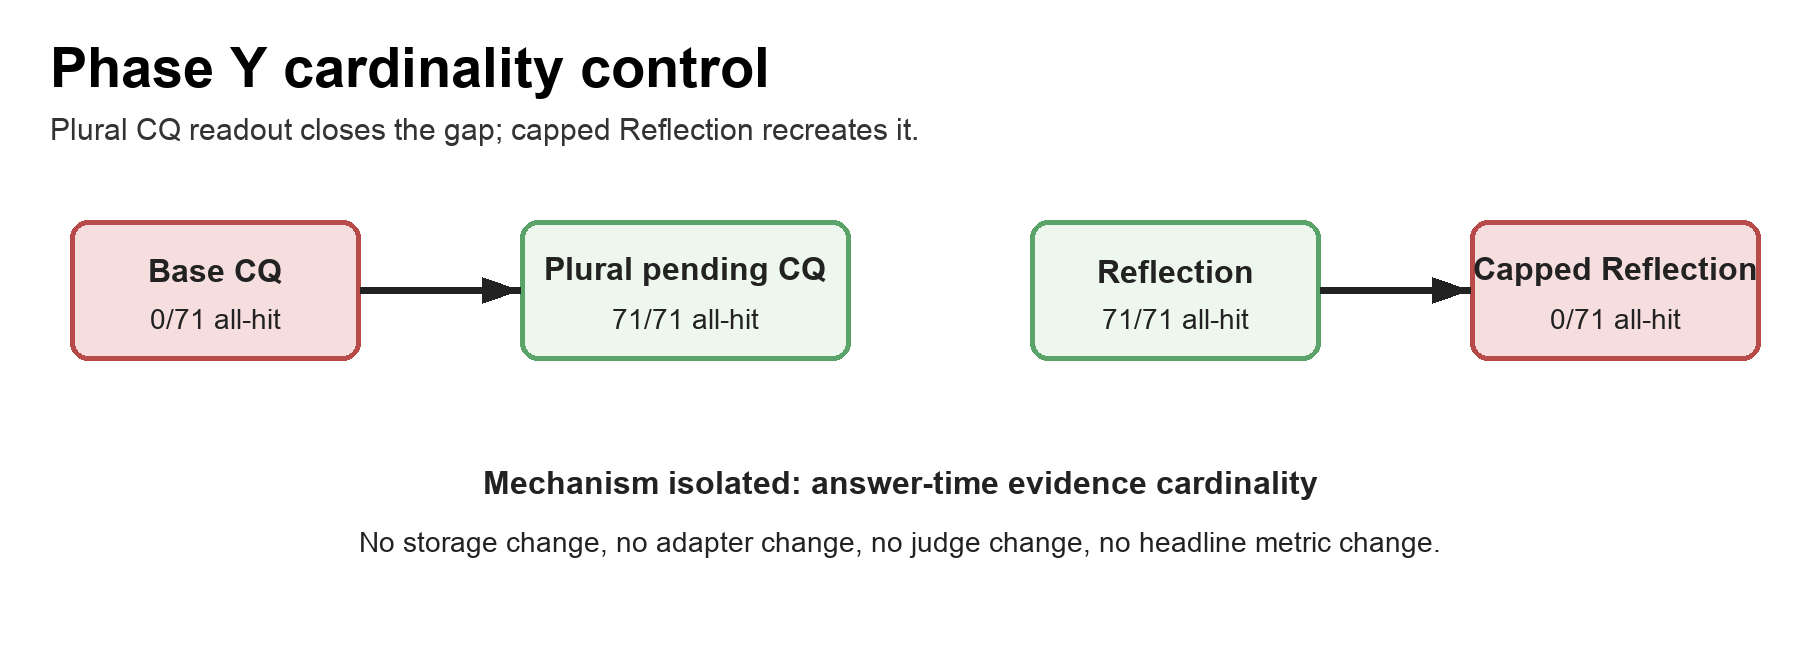
\includegraphics{figures/phase_y_cardinality_control.png}
% in paper/sections/results.tex with
%   % Cardinality-repair follow-up (repo: Phase Y; replaces phase_y_cardinality_control.png).
%
% Usage: see externalization_protocol.tex for the required preamble.
% Replace the existing 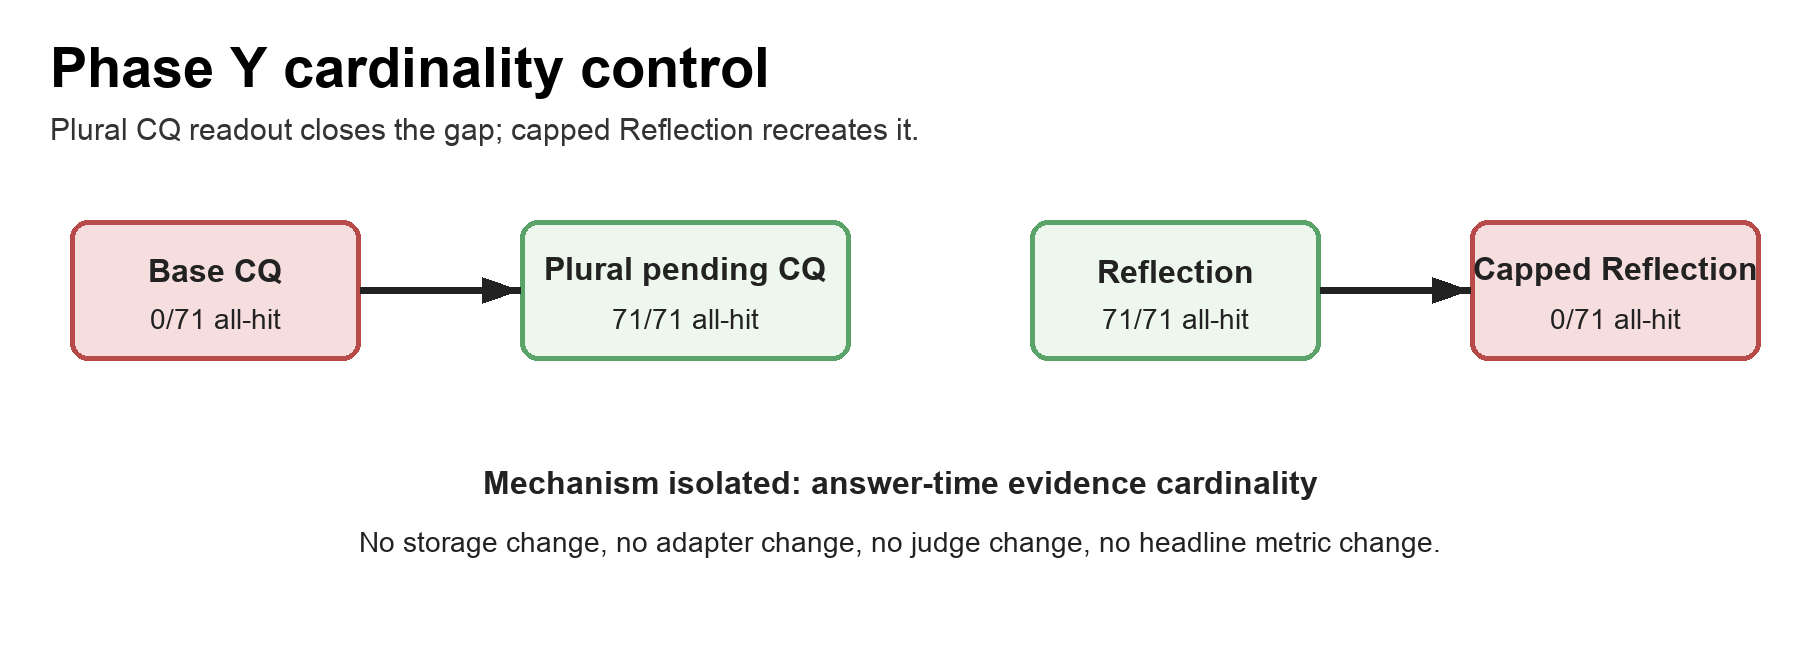
\includegraphics{figures/phase_y_cardinality_control.png}
% in paper/sections/results.tex with
%   % Cardinality-repair follow-up (repo: Phase Y; replaces phase_y_cardinality_control.png).
%
% Usage: see externalization_protocol.tex for the required preamble.
% Replace the existing 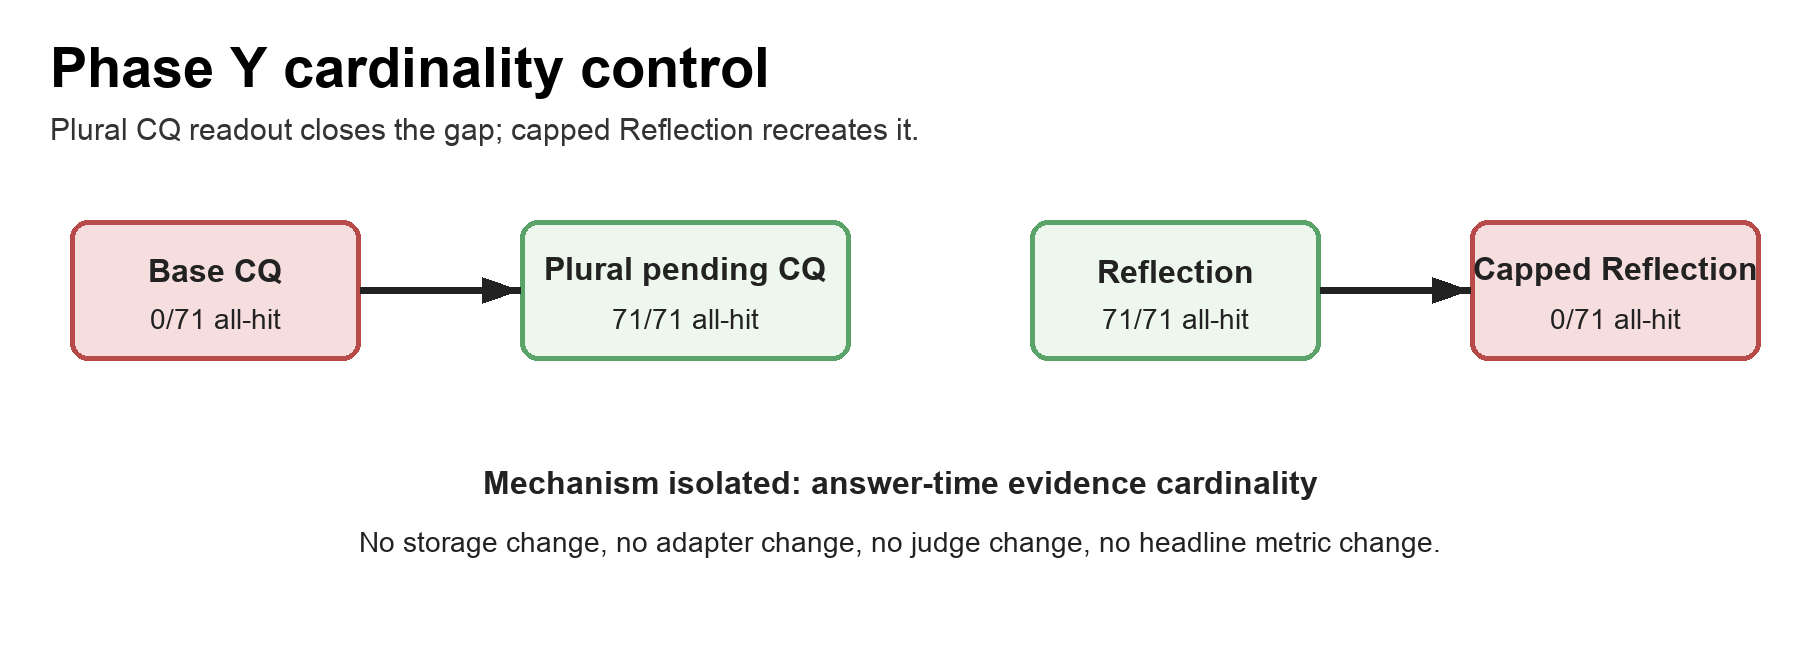
\includegraphics{figures/phase_y_cardinality_control.png}
% in paper/sections/results.tex with
%   % Cardinality-repair follow-up (repo: Phase Y; replaces phase_y_cardinality_control.png).
%
% Usage: see externalization_protocol.tex for the required preamble.
% Replace the existing 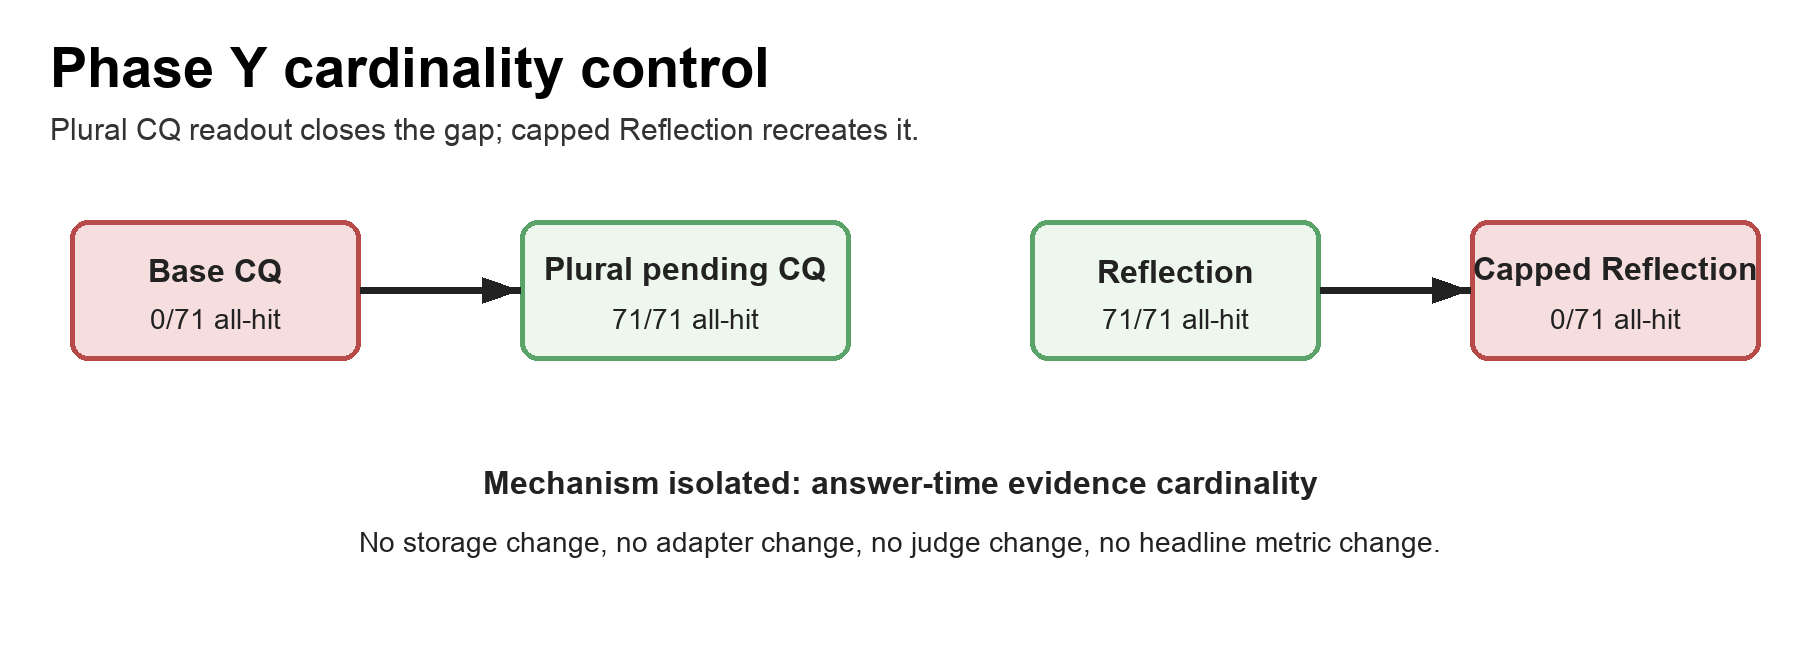
\includegraphics{figures/phase_y_cardinality_control.png}
% in paper/sections/results.tex with
%   \input{figures/phase_y_cardinality_control.tex}
%
% Sources for the depicted numbers:
%   docs/cq_pending_multi_evidence_results.md (primary_contract cell)
%   data/external/longmemeval/transfer_followup_per_case_rows.csv
%   cq/memory/cq_pending_multi_evidence.py
%   cq/memory/reflection_eager_write_cardinality_capped.py

\begin{figure}[t]
\centering
\resizebox{\linewidth}{!}{%
\begin{tikzpicture}[
  font=\small,
  node distance=6mm,
  state/.style={
    rounded corners=3pt, draw, line width=0.7pt,
    minimum width=32mm, minimum height=14mm,
    align=center, inner sep=2mm,
  },
  lose/.style={state, draw=red!60!black,   fill=red!7},
  win/.style ={state, draw=green!55!black, fill=green!8},
  swap/.style={
    -{Stealth[length=2.4mm]}, line width=0.8pt,
  },
  swaplabel/.style={
    font=\scriptsize, align=center,
    fill=white, inner sep=1pt,
  },
  caption/.style={font=\small\bfseries, align=center},
  subcap/.style={font=\footnotesize, align=center, color=black!65},
  panel/.style={
    rounded corners=4pt, draw=black!25, line width=0.4pt,
    inner sep=4mm,
  },
]

% ===== Left half: CQ swap (lose -> win) =====
\node[lose] (cq0) {\textbf{Base CQ}\\$0\,/\,71$ all\_hit\_at\_50};
\node[win, right=26mm of cq0] (cq1) {\textbf{Plural pending CQ}\\$71\,/\,71$ all\_hit\_at\_50};

\draw[swap] (cq0.east) -- node[swaplabel, above]
  {pending readout:\\[-1pt]\textbf{1} $\to$ \textbf{all eligible}}
  (cq1.west);

\node[subcap, below=2pt of cq0] {(loses completeness)};
\node[subcap, below=2pt of cq1] {(closes completeness)};

% ===== Right half: Reflection swap (win -> lose) =====
\node[win, right=44mm of cq1] (rf0) {\textbf{Reflection}\\$71\,/\,71$ all\_hit\_at\_50};
\node[lose, right=26mm of rf0] (rf1) {\textbf{Capped Reflection}\\$0\,/\,71$ all\_hit\_at\_50};

\draw[swap] (rf0.east) -- node[swaplabel, above]
  {answer readout:\\[-1pt]\textbf{all} $\to$ \textbf{1}}
  (rf1.west);

\node[subcap, below=2pt of rf0] {(wins completeness)};
\node[subcap, below=2pt of rf1] {(reproduces loss)};

% ===== Vertical separator between the two swaps =====
\draw[draw=black!20, dashed, line width=0.4pt]
  ($(cq1.east)!0.5!(rf0.west)+(0,18mm)$) -- ($(cq1.east)!0.5!(rf0.west)+(0,-32mm)$);

% ===== Section captions above each swap =====
\node[caption, above=10mm of cq0.north east, anchor=center,
      xshift=22mm] (cqcap)
  {CQ: expose plural pending evidence};
\node[caption, above=10mm of rf0.north east, anchor=center,
      xshift=22mm] (rfcap)
  {Reflection: cap durable readout to one id};

% ===== Bottom takeaway =====
\node[caption, below=18mm of cq1.south east, anchor=north, xshift=22mm]
  (takeaway) {Mechanism isolated: answer-time evidence cardinality.};
\node[subcap, below=1mm of takeaway]
  {No storage change. No adapter change. No judge change. No headline-metric change.};

\end{tikzpicture}%
}
\caption{Cardinality-repair follow-up. Changing the CQ pending-readout
  cardinality from singleton to plural converts a $0/71$ loss into a $71/71$
  win on \texttt{all\_hit\_at\_50} in the primary cell. Capping the durable
  Reflection readout to a single id reproduces the original CQ loss with the
  same magnitude. The symmetric swap isolates answer-time evidence
  cardinality as the responsible interface variable; nothing else in the
  pipeline changes.}
\label{fig:phase-y-cardinality}
\end{figure}

%
% Sources for the depicted numbers:
%   docs/cq_pending_multi_evidence_results.md (primary_contract cell)
%   data/external/longmemeval/transfer_followup_per_case_rows.csv
%   cq/memory/cq_pending_multi_evidence.py
%   cq/memory/reflection_eager_write_cardinality_capped.py

\begin{figure}[t]
\centering
\resizebox{\linewidth}{!}{%
\begin{tikzpicture}[
  font=\small,
  node distance=6mm,
  state/.style={
    rounded corners=3pt, draw, line width=0.7pt,
    minimum width=32mm, minimum height=14mm,
    align=center, inner sep=2mm,
  },
  lose/.style={state, draw=red!60!black,   fill=red!7},
  win/.style ={state, draw=green!55!black, fill=green!8},
  swap/.style={
    -{Stealth[length=2.4mm]}, line width=0.8pt,
  },
  swaplabel/.style={
    font=\scriptsize, align=center,
    fill=white, inner sep=1pt,
  },
  caption/.style={font=\small\bfseries, align=center},
  subcap/.style={font=\footnotesize, align=center, color=black!65},
  panel/.style={
    rounded corners=4pt, draw=black!25, line width=0.4pt,
    inner sep=4mm,
  },
]

% ===== Left half: CQ swap (lose -> win) =====
\node[lose] (cq0) {\textbf{Base CQ}\\$0\,/\,71$ all\_hit\_at\_50};
\node[win, right=26mm of cq0] (cq1) {\textbf{Plural pending CQ}\\$71\,/\,71$ all\_hit\_at\_50};

\draw[swap] (cq0.east) -- node[swaplabel, above]
  {pending readout:\\[-1pt]\textbf{1} $\to$ \textbf{all eligible}}
  (cq1.west);

\node[subcap, below=2pt of cq0] {(loses completeness)};
\node[subcap, below=2pt of cq1] {(closes completeness)};

% ===== Right half: Reflection swap (win -> lose) =====
\node[win, right=44mm of cq1] (rf0) {\textbf{Reflection}\\$71\,/\,71$ all\_hit\_at\_50};
\node[lose, right=26mm of rf0] (rf1) {\textbf{Capped Reflection}\\$0\,/\,71$ all\_hit\_at\_50};

\draw[swap] (rf0.east) -- node[swaplabel, above]
  {answer readout:\\[-1pt]\textbf{all} $\to$ \textbf{1}}
  (rf1.west);

\node[subcap, below=2pt of rf0] {(wins completeness)};
\node[subcap, below=2pt of rf1] {(reproduces loss)};

% ===== Vertical separator between the two swaps =====
\draw[draw=black!20, dashed, line width=0.4pt]
  ($(cq1.east)!0.5!(rf0.west)+(0,18mm)$) -- ($(cq1.east)!0.5!(rf0.west)+(0,-32mm)$);

% ===== Section captions above each swap =====
\node[caption, above=10mm of cq0.north east, anchor=center,
      xshift=22mm] (cqcap)
  {CQ: expose plural pending evidence};
\node[caption, above=10mm of rf0.north east, anchor=center,
      xshift=22mm] (rfcap)
  {Reflection: cap durable readout to one id};

% ===== Bottom takeaway =====
\node[caption, below=18mm of cq1.south east, anchor=north, xshift=22mm]
  (takeaway) {Mechanism isolated: answer-time evidence cardinality.};
\node[subcap, below=1mm of takeaway]
  {No storage change. No adapter change. No judge change. No headline-metric change.};

\end{tikzpicture}%
}
\caption{Cardinality-repair follow-up. Changing the CQ pending-readout
  cardinality from singleton to plural converts a $0/71$ loss into a $71/71$
  win on \texttt{all\_hit\_at\_50} in the primary cell. Capping the durable
  Reflection readout to a single id reproduces the original CQ loss with the
  same magnitude. The symmetric swap isolates answer-time evidence
  cardinality as the responsible interface variable; nothing else in the
  pipeline changes.}
\label{fig:phase-y-cardinality}
\end{figure}

%
% Sources for the depicted numbers:
%   docs/cq_pending_multi_evidence_results.md (primary_contract cell)
%   data/external/longmemeval/transfer_followup_per_case_rows.csv
%   cq/memory/cq_pending_multi_evidence.py
%   cq/memory/reflection_eager_write_cardinality_capped.py

\begin{figure}[t]
\centering
\resizebox{\linewidth}{!}{%
\begin{tikzpicture}[
  font=\small,
  node distance=6mm,
  state/.style={
    rounded corners=3pt, draw, line width=0.7pt,
    minimum width=32mm, minimum height=14mm,
    align=center, inner sep=2mm,
  },
  lose/.style={state, draw=red!60!black,   fill=red!7},
  win/.style ={state, draw=green!55!black, fill=green!8},
  swap/.style={
    -{Stealth[length=2.4mm]}, line width=0.8pt,
  },
  swaplabel/.style={
    font=\scriptsize, align=center,
    fill=white, inner sep=1pt,
  },
  caption/.style={font=\small\bfseries, align=center},
  subcap/.style={font=\footnotesize, align=center, color=black!65},
  panel/.style={
    rounded corners=4pt, draw=black!25, line width=0.4pt,
    inner sep=4mm,
  },
]

% ===== Left half: CQ swap (lose -> win) =====
\node[lose] (cq0) {\textbf{Base CQ}\\$0\,/\,71$ all\_hit\_at\_50};
\node[win, right=26mm of cq0] (cq1) {\textbf{Plural pending CQ}\\$71\,/\,71$ all\_hit\_at\_50};

\draw[swap] (cq0.east) -- node[swaplabel, above]
  {pending readout:\\[-1pt]\textbf{1} $\to$ \textbf{all eligible}}
  (cq1.west);

\node[subcap, below=2pt of cq0] {(loses completeness)};
\node[subcap, below=2pt of cq1] {(closes completeness)};

% ===== Right half: Reflection swap (win -> lose) =====
\node[win, right=44mm of cq1] (rf0) {\textbf{Reflection}\\$71\,/\,71$ all\_hit\_at\_50};
\node[lose, right=26mm of rf0] (rf1) {\textbf{Capped Reflection}\\$0\,/\,71$ all\_hit\_at\_50};

\draw[swap] (rf0.east) -- node[swaplabel, above]
  {answer readout:\\[-1pt]\textbf{all} $\to$ \textbf{1}}
  (rf1.west);

\node[subcap, below=2pt of rf0] {(wins completeness)};
\node[subcap, below=2pt of rf1] {(reproduces loss)};

% ===== Vertical separator between the two swaps =====
\draw[draw=black!20, dashed, line width=0.4pt]
  ($(cq1.east)!0.5!(rf0.west)+(0,18mm)$) -- ($(cq1.east)!0.5!(rf0.west)+(0,-32mm)$);

% ===== Section captions above each swap =====
\node[caption, above=10mm of cq0.north east, anchor=center,
      xshift=22mm] (cqcap)
  {CQ: expose plural pending evidence};
\node[caption, above=10mm of rf0.north east, anchor=center,
      xshift=22mm] (rfcap)
  {Reflection: cap durable readout to one id};

% ===== Bottom takeaway =====
\node[caption, below=18mm of cq1.south east, anchor=north, xshift=22mm]
  (takeaway) {Mechanism isolated: answer-time evidence cardinality.};
\node[subcap, below=1mm of takeaway]
  {No storage change. No adapter change. No judge change. No headline-metric change.};

\end{tikzpicture}%
}
\caption{Cardinality-repair follow-up. Changing the CQ pending-readout
  cardinality from singleton to plural converts a $0/71$ loss into a $71/71$
  win on \texttt{all\_hit\_at\_50} in the primary cell. Capping the durable
  Reflection readout to a single id reproduces the original CQ loss with the
  same magnitude. The symmetric swap isolates answer-time evidence
  cardinality as the responsible interface variable; nothing else in the
  pipeline changes.}
\label{fig:phase-y-cardinality}
\end{figure}

%
% Sources for the depicted numbers:
%   docs/cq_pending_multi_evidence_results.md (primary_contract cell)
%   data/external/longmemeval/transfer_followup_per_case_rows.csv
%   cq/memory/cq_pending_multi_evidence.py
%   cq/memory/reflection_eager_write_cardinality_capped.py

\begin{figure}[t]
\centering
\resizebox{\linewidth}{!}{%
\begin{tikzpicture}[
  font=\small,
  node distance=6mm,
  state/.style={
    rounded corners=3pt, draw, line width=0.7pt,
    minimum width=32mm, minimum height=14mm,
    align=center, inner sep=2mm,
  },
  lose/.style={state, draw=red!60!black,   fill=red!7},
  win/.style ={state, draw=green!55!black, fill=green!8},
  swap/.style={
    -{Stealth[length=2.4mm]}, line width=0.8pt,
  },
  swaplabel/.style={
    font=\scriptsize, align=center,
    fill=white, inner sep=1pt,
  },
  caption/.style={font=\small\bfseries, align=center},
  subcap/.style={font=\footnotesize, align=center, color=black!65},
  panel/.style={
    rounded corners=4pt, draw=black!25, line width=0.4pt,
    inner sep=4mm,
  },
]

% ===== Left half: CQ swap (lose -> win) =====
\node[lose] (cq0) {\textbf{Base CQ}\\$0\,/\,71$ all\_hit\_at\_50};
\node[win, right=26mm of cq0] (cq1) {\textbf{Plural pending CQ}\\$71\,/\,71$ all\_hit\_at\_50};

\draw[swap] (cq0.east) -- node[swaplabel, above]
  {pending readout:\\[-1pt]\textbf{1} $\to$ \textbf{all eligible}}
  (cq1.west);

\node[subcap, below=2pt of cq0] {(loses completeness)};
\node[subcap, below=2pt of cq1] {(closes completeness)};

% ===== Right half: Reflection swap (win -> lose) =====
\node[win, right=44mm of cq1] (rf0) {\textbf{Reflection}\\$71\,/\,71$ all\_hit\_at\_50};
\node[lose, right=26mm of rf0] (rf1) {\textbf{Capped Reflection}\\$0\,/\,71$ all\_hit\_at\_50};

\draw[swap] (rf0.east) -- node[swaplabel, above]
  {answer readout:\\[-1pt]\textbf{all} $\to$ \textbf{1}}
  (rf1.west);

\node[subcap, below=2pt of rf0] {(wins completeness)};
\node[subcap, below=2pt of rf1] {(reproduces loss)};

% ===== Vertical separator between the two swaps =====
\draw[draw=black!20, dashed, line width=0.4pt]
  ($(cq1.east)!0.5!(rf0.west)+(0,18mm)$) -- ($(cq1.east)!0.5!(rf0.west)+(0,-32mm)$);

% ===== Section captions above each swap =====
\node[caption, above=10mm of cq0.north east, anchor=center,
      xshift=22mm] (cqcap)
  {CQ: expose plural pending evidence};
\node[caption, above=10mm of rf0.north east, anchor=center,
      xshift=22mm] (rfcap)
  {Reflection: cap durable readout to one id};

% ===== Bottom takeaway =====
\node[caption, below=18mm of cq1.south east, anchor=north, xshift=22mm]
  (takeaway) {Mechanism isolated: answer-time evidence cardinality.};
\node[subcap, below=1mm of takeaway]
  {No storage change. No adapter change. No judge change. No headline-metric change.};

\end{tikzpicture}%
}
\caption{Cardinality-repair follow-up. Changing the CQ pending-readout
  cardinality from singleton to plural converts a $0/71$ loss into a $71/71$
  win on \texttt{all\_hit\_at\_50} in the primary cell. Capping the durable
  Reflection readout to a single id reproduces the original CQ loss with the
  same magnitude. The symmetric swap isolates answer-time evidence
  cardinality as the responsible interface variable; nothing else in the
  pipeline changes.}
\label{fig:phase-y-cardinality}
\end{figure}
